\documentclass[aspectratio=169,notes]{beamer}
% \documentclass[aspectratio=169]{beamer}
\usetheme[faculty=phil]{fibeamer}
\usepackage{polyglossia}
\setmainlanguage{english} %% main locale instead of `english`, you
%% can typeset the presentation in either Czech or Slovak,
%% respectively.
\setotherlanguages{russian} %% The additional keys allow
%%
%%   \begin{otherlanguage}{czech}   ... \end{otherlanguage}
%%   \begin{otherlanguage}{slovak}  ... \end{otherlanguage}
%%
%% These macros specify information about the presentation
\title[AGLA1]{Analytical Geometry and Linear Algebra I, Lab 1} %% that will be typeset on the
\subtitle{Introduction to AGLA \\ Vector  \\ Basis and Subspace  
         } %% title page.
\author{Oleg Bulichev}
%% These additional packages are used within the document:
\usepackage{ragged2e}  % `\justifying` text
\usepackage{booktabs}  % Tables
\usepackage{tabularx}
\usepackage{tikz}      % Diagrams
\usetikzlibrary{calc, shapes, backgrounds}
\usepackage{amsmath, amssymb}
\usepackage{url}       % `\url`s
\usepackage{listings}  % Code listings
% \usepackage{subfigure}
\usepackage{floatrow}
\usepackage{subcaption}
\usepackage{mathtools}
\usepackage{todonotes}
\usepackage{fontspec}
\usepackage{multicol}
\usepackage{pdfpages}
\usepackage{wrapfig}
\usepackage{animate}
\usepackage{booktabs}
\usepackage{multirow}

\graphicspath{{resources/}}
\frenchspacing

\setbeamertemplate{caption}[numbered]
\usetikzlibrary{graphs}

% \usepackage[backend=biber,style=ieee,autocite=footnote]{biblatex}
% \addbibresource{biblio.bib}
% \DefineBibliographyStrings{english}{%
%   bibliography = {References},}

\newcommand{\oleg}[2][] {\todo[color=red, #1] {OLEG:\\ #2}}
\newcommand{\fbckg}[1]{\usebackgroundtemplate{\includegraphics[width=\paperwidth]{#1}}}%frame background

\usepackage[framemethod=TikZ]{mdframed}
\newcommand{\dbox}[1]{
\begin{mdframed}[roundcorner=3pt, backgroundcolor=yellow, linewidth=0]
\vspace{1mm}
{#1}
\vspace{1mm}
\end{mdframed}
}

\begin{document}
\setlength{\abovedisplayskip}{0pt}
\setlength{\belowdisplayskip}{0pt}
\setlength{\abovedisplayshortskip}{0pt}
\setlength{\belowdisplayshortskip}{0pt}

\fbckg{fibeamer/figs/title_page.png}
\frame[c]{\setcounter{framenumber}{0}
    \usebeamerfont{title}%
    \usebeamercolor[fg]{title}%
    \begin{minipage}[b][6.5\baselineskip][b]{\textwidth}%
        \textcolor{black}{\raggedright\inserttitle}
    \end{minipage}
    % \vskip-1.5\baselineskip

    \usebeamerfont{subtitle}%
    \usebeamercolor[fg]{framesubtitle}%
    \begin{minipage}[b][3\baselineskip][b]{\textwidth}
        \raggedright%
        \insertsubtitle%
    \end{minipage}
    \vskip.25\baselineskip
}
%   \frame[c]{\maketitle}

\fbckg{fibeamer/figs/common.png}

\begin{frame}[t]{About Me (1)}
    \framesubtitle{}
    \begin{columns}[T,onlytextwidth]
        \begin{column}{0.49\textwidth}
            \begin{figure}[H]
                \centering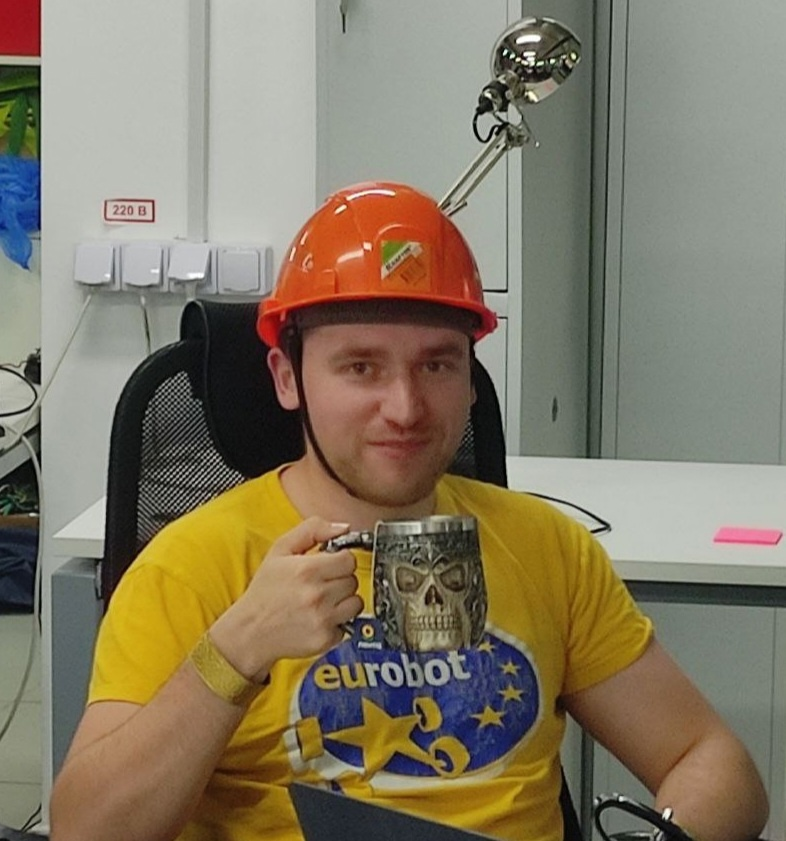
\includegraphics[height=5cm,width=1\textwidth,keepaspectratio]{Oleg.jpg}
                % \caption{caption_name}
                \label{fig:Oleg.jpg}
            \end{figure}
        \end{column}
        \begin{column}{0.49\textwidth}
            \Large
            \vspace{2cm}
            \centering
            \textbf{Oleg Bulichev} \\
            \textit{Mail}: \url{o.bulichev@innopolis.ru}\\
            \textit{TG}: \url{@Lupasic} \\
            \textit{Office Hours}: By request
        \end{column}
    \end{columns}
\end{frame}

\begin{frame}[t]{About Me (2)}
    \framesubtitle{}
    \begin{columns}[T,onlytextwidth]
        \begin{column}{0.69\textwidth}
            \textbf{Education}
            \begin{itemize}
                \item \textit{Bachelor} --- BMSTU (МГТУ им Н.Э. Баумана) <<CAD developer>>
                \item \textit{Master \& PHD} --- Innopolis University (IU) <<Robotics>>
            \end{itemize}
            \textbf{Job}
            \begin{itemize}
                \item \textit{Senior Lecturer} --- IU: Linear Algebra, Theoretical Mechanics, Mechanics and Machines
                \item \textit{Course Author} --- Skillbox: Mathematics for Robotics
                \item \textit{Trainer} --- IU: RAGE (ДИЧь) club -- Hiking / Kayaking, Historical fencing, Folkgames, Archery
            \end{itemize}
        \end{column}
        \begin{column}{0.29\textwidth}
            \begin{figure}[H]
                \centering
\includegraphics[height=6cm,width=1\textwidth,keepaspectratio]{resources/image2.png}
                \caption*{\href{https://t.me/dich_trainings}{\textbf{Link to the channel}}}
                \label{fig:resources/image2.png}
            \end{figure}
        \end{column}
    \end{columns}
\end{frame}

\begin{frame}[t]{Where did I use linear algebra?}
    \framesubtitle{Problem 1}
    \vspace{-0.3cm}
    \begin{columns}[T,onlytextwidth]
        \begin{column}{0.34\textwidth}
            To determine geometrical and physical properties of passed terrain. \medskip

            \textbf{Linear Algebra topics:}
            \begin{itemize}
                \item All core topics from LA (vector, matrix, etc)
                \item Change of basis
                \item Projections, regression
            \end{itemize}
        \end{column}
        \begin{column}{0.64\textwidth}
            \vspace{-0.4cm}
            \begin{figure}[H]
                \begin{subfigure}{0.49\textwidth}
                    \centering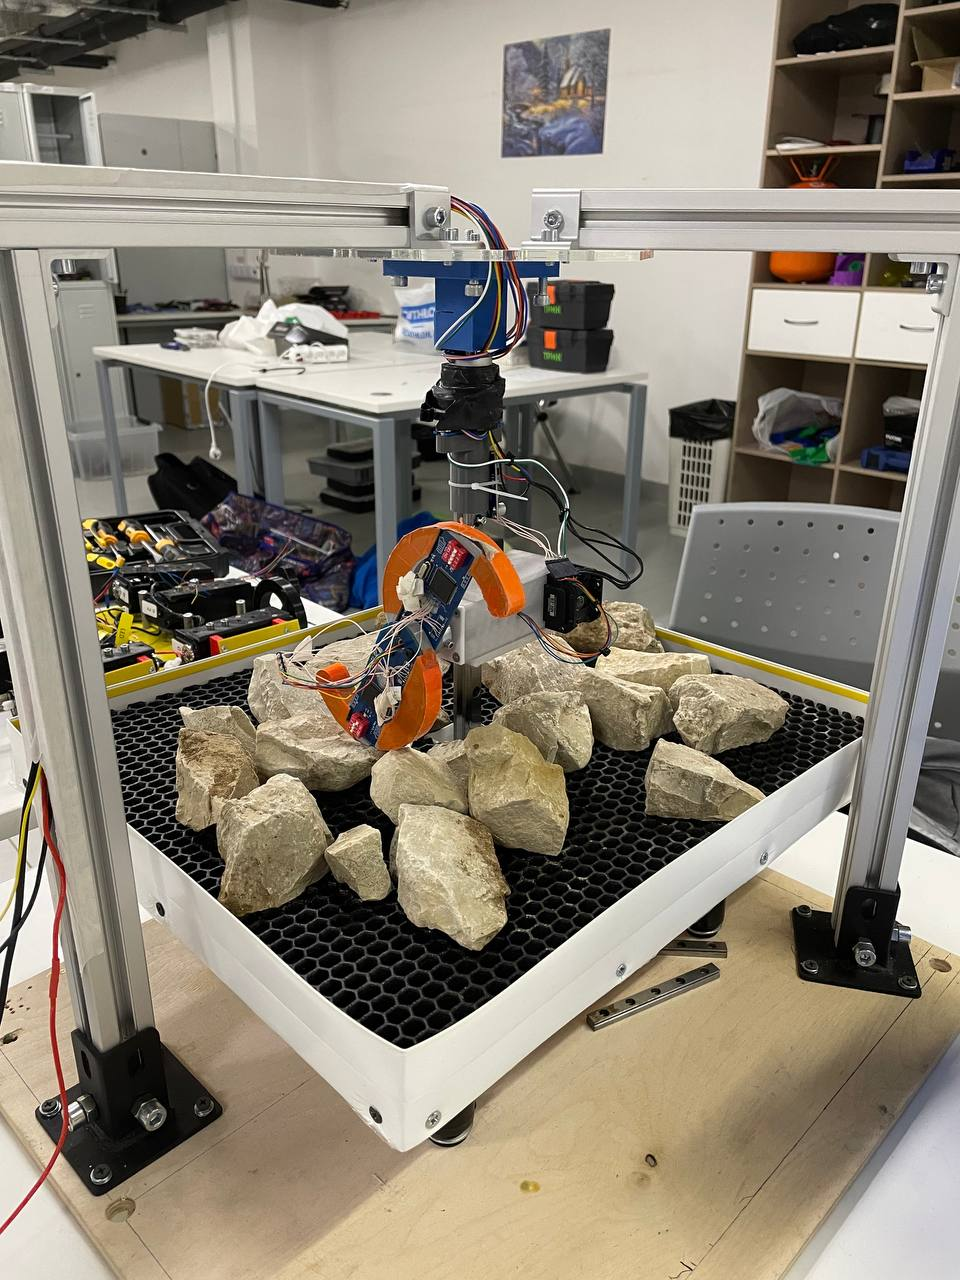
\includegraphics[height=5.5cm,width=1\textwidth,keepaspectratio]{resources/view.jpg}
                    \label{fig:resources/view.jpg}
                \end{subfigure}
                \begin{subfigure}{0.49\textwidth}
                    \centering\includegraphics[height=5.5cm,width=1\textwidth,keepaspectratio]{resources/rl_sims.png}
                    \label{fig:resources/rl_sims.png}
                \end{subfigure}
            \end{figure}
        \end{column}
    \end{columns}
\end{frame}

\begin{frame}[t]{Where did I use linear algebra?}
    \framesubtitle{Problem 2}
    \vspace{-0.3cm}
    \begin{columns}[T,onlytextwidth]
        \begin{column}{0.34\textwidth}
            To determine the position and orientation of a mug using camera. \medskip

            \textbf{Linear Algebra topics:}
            \begin{itemize}
                \item All core topics from LA (vector, matrix, etc)
                \item Change of basis, affine transformations
                \item Projections
            \end{itemize}
        \end{column}
        \begin{column}{0.64\textwidth}
            \vspace{-0.4cm}
            \begin{figure}[H]
                \begin{subfigure}[c]{0.49\textwidth}
                    \centering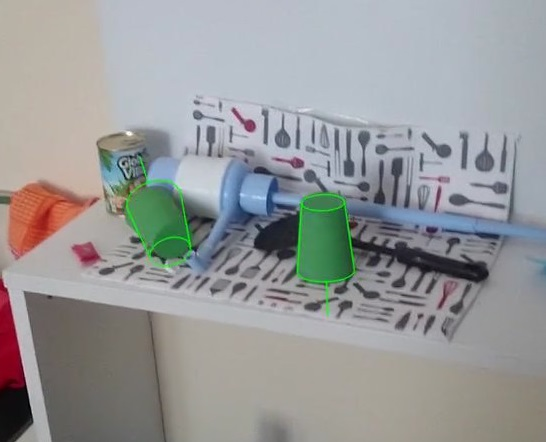
\includegraphics[height=6cm,width=1\textwidth,keepaspectratio]{resources/output_Moment.jpg}
                    \label{fig:resources/output_Moment.jpg}
                \end{subfigure}
                \begin{subfigure}[c]{0.49\textwidth}
                    \centering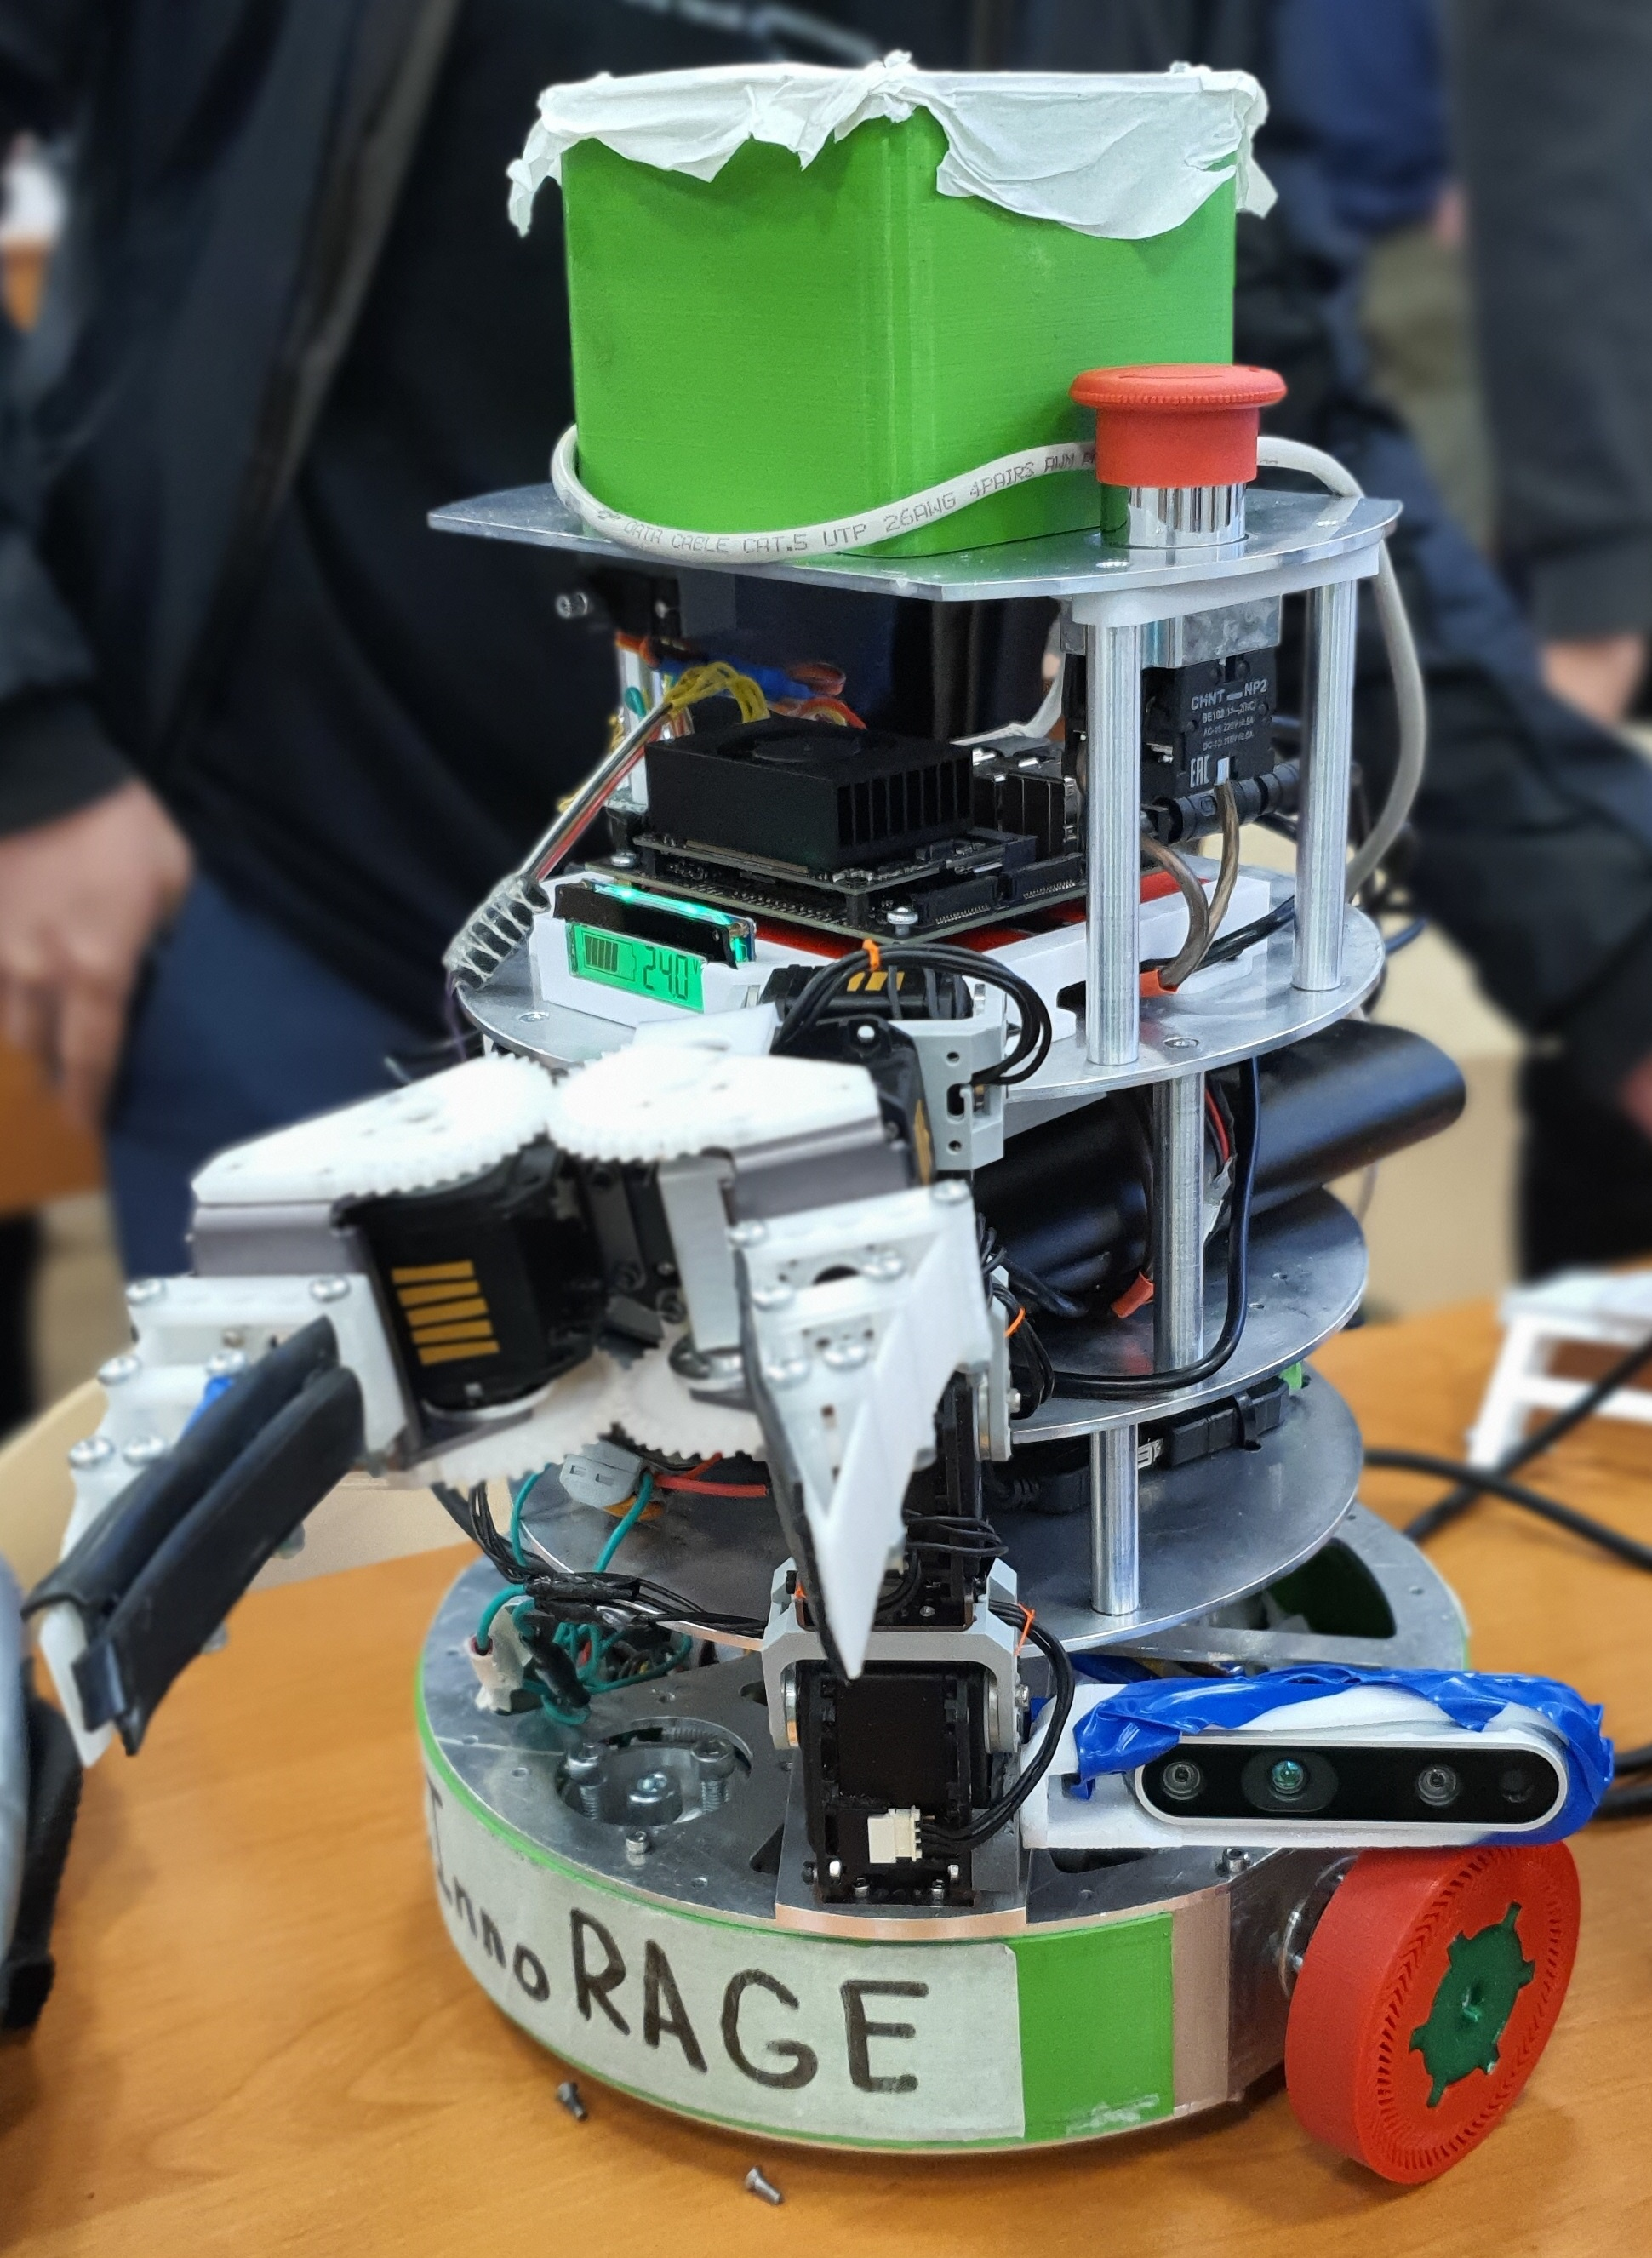
\includegraphics[height=6cm,width=1\textwidth,keepaspectratio]{resources/2021-05-21 14-08-47.JPG}
                    \label{fig:resources/2021-05-21 14-08-47.JPG}
                \end{subfigure}
            \end{figure}
        \end{column}
    \end{columns}
\end{frame}

\begin{frame}[t]{Where did I use linear algebra?}
    \framesubtitle{Problem 3}
    \vspace{-0.3cm}
    \begin{columns}[T,onlytextwidth]
        \begin{column}{0.34\textwidth}
            To simulate the mechanism. \medskip

            \textbf{Linear Algebra topics:}
            \begin{itemize}
                \item Vectors, Matrices
                \item Change of basis
            \end{itemize}
        \end{column}
        \begin{column}{0.64\textwidth}
            \vspace{-0.4cm}
            \begin{figure}[H]
                \href{https://drive.google.com/file/d/1vQFNiLfshH4hhh-Kb0mHS-fJaC5o_RsH/view}{
                    \centering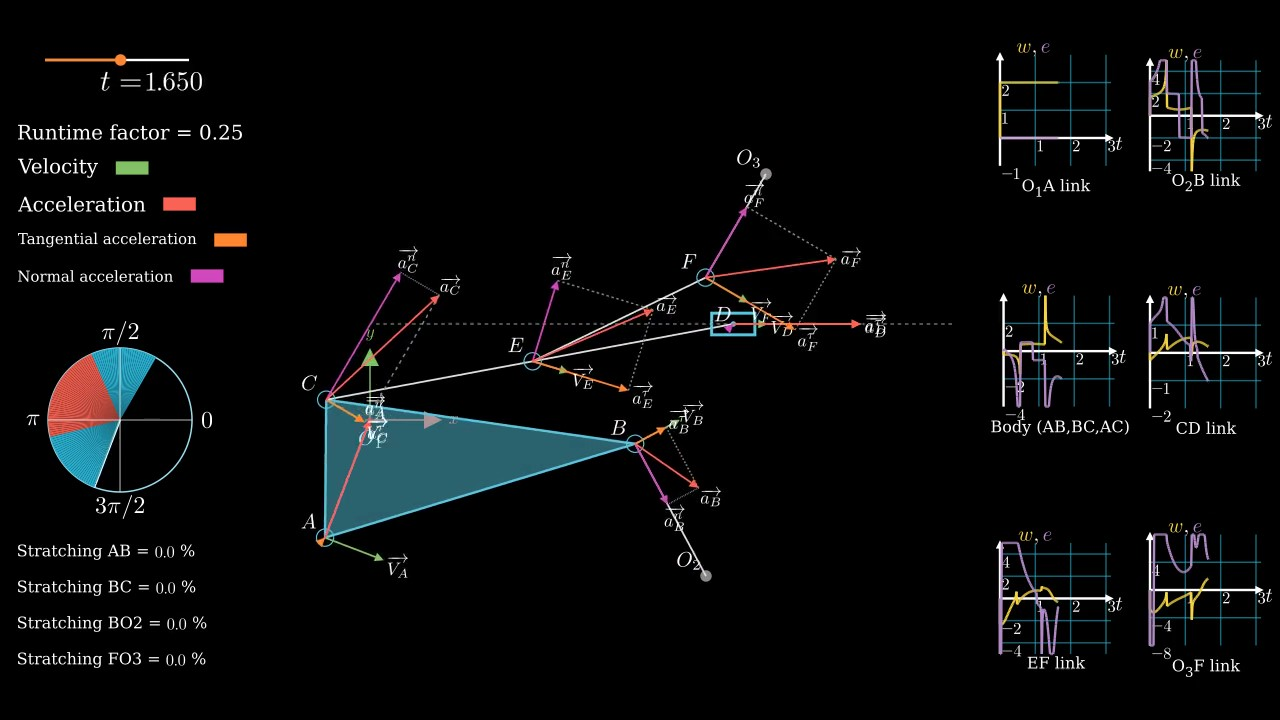
\includegraphics[height=6cm,width=1\textwidth,keepaspectratio]{resources/doc.jpg}}
                \label{fig:resources/doc.jpg}
            \end{figure}
        \end{column}
    \end{columns}
\end{frame}

\begin{frame}[t]{Short Summary}
    \framesubtitle{}
    \begin{enumerate}
        \item I used to use the course knowledge in my research career
        \item It's not a useless course and I'll try to show it by presenting practical cases (not only from robotics))
        \item I will give you an intuition of some basics
    \end{enumerate}
\end{frame}

\begin{frame}[c]{}
    \framesubtitle{}
    \centering\LARGE
    \textbf{Agreements among the group (for now)}
\end{frame}

\begin{frame}[t]{Pretest}
    \framesubtitle{}
    \LARGE
    \begin{multicols}{2}
        \begin{itemize}
            \item Vector
            \item Span
            \item Linear combination
            \item Linear independence
            \item Vector length
            \item Subspace
        \end{itemize}
    \end{multicols}
\end{frame}

\begin{frame}[t]{Vector}
    \framesubtitle{Definition from school}
    \begin{columns}[T,onlytextwidth]
        \begin{column}{0.49\textwidth}
            In the simplest case, it is a mathematical object characterized by magnitude and direction.

            It is a directed segment with a certain length.
        \end{column}
        \begin{column}{0.49\textwidth}
            \begin{figure}[H]
                \centering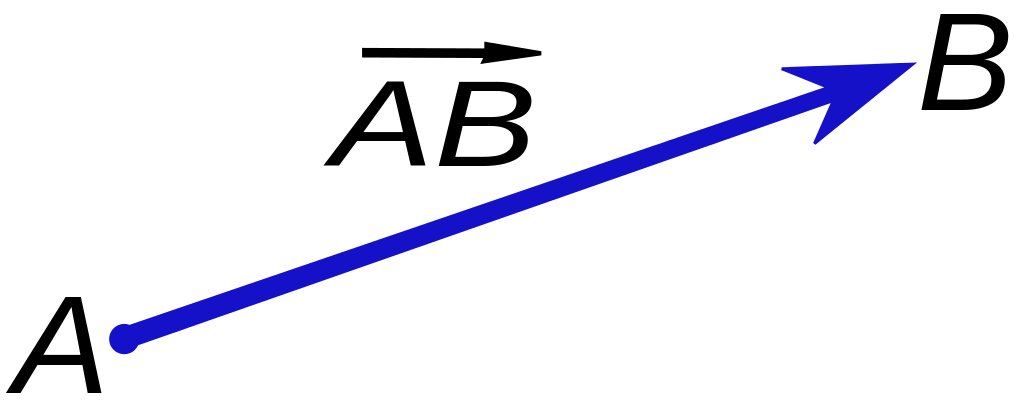
\includegraphics[height=6cm,width=1\textwidth,keepaspectratio]{resources/Vector_AB_from_A_to_B.svg.png}
                % \caption{caption_name}
                \label{fig:resources/Vector_AB_from_A_to_B.svg.png}
            \end{figure}
        \end{column}
    \end{columns}
\end{frame}

\begin{frame}[t]{How a vector is seen by}
    \framesubtitle{}
    \vspace{-0.6cm}
    \begin{figure}[H]
        \centering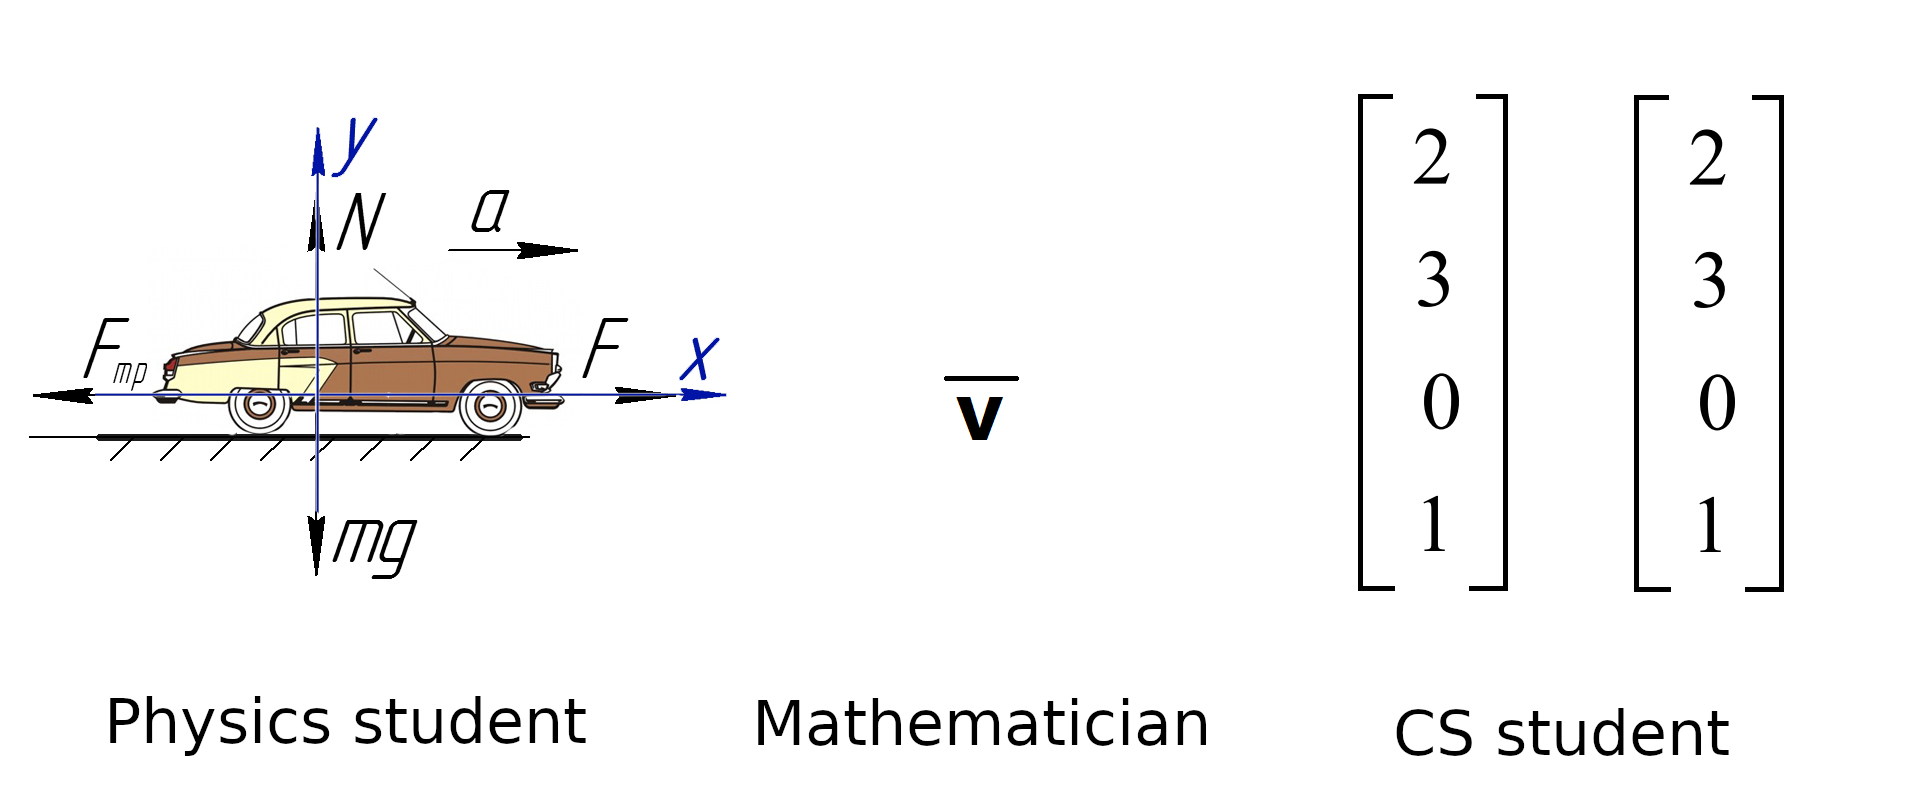
\includegraphics[height=6cm,width=1\textwidth,keepaspectratio]{resources/Vector_representation.png}
        \label{fig:file_name}
    \end{figure}
\end{frame}

\begin{frame}[t]{Vector operations}
    \framesubtitle{}
    \begin{itemize}
        \item Summation
        \item Scalar multiplication
        \item Norm / magnitude / vector length
        \item Transpose
        \item Dot (inner) product
        \item Cross (outer) product
    \end{itemize}
\end{frame}

\begin{frame}[t]{Task 1}
    \framesubtitle{}
    We have $\vec{a} = \begin{bmatrix}
            1 \\ 2
        \end{bmatrix}$, $\vec{b} = \begin{bmatrix}
            -5 \\ -1
        \end{bmatrix}$, $\vec{c} = \begin{bmatrix}
            -1 \\ 3
        \end{bmatrix}$.
    \medskip

    You should find $2\vec{a} + 3\vec{b} - \vec{c}$ и $16\vec{a} + 5\vec{b} - 9\vec{c}$
\end{frame}

\begin{frame}[t]{Task 2}
    \framesubtitle{}
    Check if the result of each of the following operations is a vector or not. Explain your answer. \\
    1. $\mathbf{a} + \mathbf{b}$, if $\mathbf{a}$ and $\mathbf{b}$ are vectors \\
    2. $\mathbf{a} - \mathbf{a}$, if $\mathbf{a}$ is a vector \\
    3.$\begin{bmatrix}
            1 \\
            0
        \end{bmatrix}
        +
        \begin{bmatrix}
            0 \\
            2
        \end{bmatrix}$ \\
    4. $\begin{bmatrix}
            2x + 15 - 4y \\
            y - x
        \end{bmatrix}$, if $x$ and $y$ are integer numbers \\
    5. $\begin{bmatrix}
            x + y \\
            2y + 122 - 3x
        \end{bmatrix} -
        \begin{bmatrix}
            x + y \\
            2y + 122 - 3x
        \end{bmatrix}$, if $x$ and $y$ are real numbers
\end{frame}

\begin{frame}{Linear combination}
    Vector $\vec{w}\in V$ is a \underline{linear combination} of $\vec{v}_1, \ldots, \vec{v}_n \in V$ vectors,

    if $\exists c_k\in \mathbb{R}; (k=1..n)$

    such as,
    \[ \vec{w} = c_1 \vec{v}_1 + c_2 \vec{v}_2 + \cdots + c_n \vec{v}_n \]

\end{frame}

\begin{frame}{Linear indepence}
    Two vectors  $\vec{a}$ и $\vec{b}$ are \emph{linear independent}

    if for $\alpha_1, \alpha_2\in \mathbb{R}$, $\alpha_1\vec{a} + \alpha_2\vec{b} = \mathbf{0}$ if and only if $\alpha_1 = \alpha_2 = 0$.

\end{frame}

\begin{frame}[t]{Span}
    \framesubtitle{}
    Let $S=\{\mathbf{v_1,v_2,\ldots, v_n\}}\subset V$.
    \[
        span (S) \equiv
        \left\{ \mathbf{w} \in V: \mathbf{w}=\sum_{k=1}^n c_k \mathbf{v_k}, \quad
        \forall c_k\in \mathbb{R}\right\}
    \] \bigskip 

    
    In words, $W=span(S)$ is the set of all (possible) linear
    combinations of the vectors $\mathbf{v_1,v_2,\ldots, v_n}$.


    Note that $W$ is a subspace of $V$.

\end{frame}

\begin{frame}{Basis}
    \vspace*{-0.5cm}
    {A \textbf{set} of vectors is a \textit{basis} of $\mathbb{R}^2$} if it spans $\mathbb{R}^2$ and this set is \textbf{linear independent}.

    \begin{exampleblock}{Standard basis in $\mathbb{R}^2$}
        $\{{\vec{i}}, {\vec{j}}\} = \{\begin{bmatrix}
                1 \\ 0
            \end{bmatrix}, \begin{bmatrix}
                0 \\ 1
            \end{bmatrix}\}$ --- is basis of $\mathbb{R}^2$. It's a classical (canonical) basis in $\mathbb{R}^2$.
    \end{exampleblock}

    \begin{exampleblock}{Standard basis in $\mathbb{R}^3$}
        $\{{\vec{i}}, {\vec{j}}, {\vec{k}}\} = \{\begin{bmatrix} 1 \\ 0 \\ 0 \end{bmatrix}, \begin{bmatrix} 0 \\ 1 \\ 0 \end{bmatrix}, \begin{bmatrix} 0 \\ 0 \\ 1 \end{bmatrix}\}$ --- basis in $\mathbb{R}^3$.
    \end{exampleblock}
\end{frame}

\begin{frame}[t]{Task 3}
    \framesubtitle{}

    \only<1>{Check for each case if the following set of vectors is a basis or not. Explain your answer. \\}
    \only<2>{\alert{\Large Answer}

        A \textbf{set} of vectors is a \textit{basis} of $\mathbb{R}^2$ if it spans $\mathbb{R}^2$ and this set is \textbf{linear independent}.}
    \begin{multicols}{2}
        \begin{enumerate}
            \item $\begin{bmatrix}
                          1 \\
                          0
                      \end{bmatrix}
                      +
                      \begin{bmatrix}
                          0 \\
                          2
                      \end{bmatrix}$ \uncover<2->{\alert{NOT}}
            \item $\begin{bmatrix}
                          1 \\
                          0
                      \end{bmatrix}$, $\begin{bmatrix}
                          0 \\
                          2
                      \end{bmatrix}$
            \item $\begin{bmatrix}
                          1 \\
                          2 \\
                          3
                      \end{bmatrix}$ \uncover<2->{\alert{NOT}}
            \item $\begin{bmatrix}
                          1 \\
                          0 \\
                          0
                      \end{bmatrix}$ ,
                  $\begin{bmatrix}
                          0 \\
                          2 \\
                          0
                      \end{bmatrix}$ ,
                  $\begin{bmatrix}
                          0 \\
                          0 \\
                          3
                      \end{bmatrix}$
            \item $\begin{bmatrix}
                          1 \\
                          0 \\
                          0
                      \end{bmatrix}$ ,
                  $\begin{bmatrix}
                          0 \\
                          2 \\
                          0
                      \end{bmatrix}$ \uncover<2->{\alert{NOT}}
            \item $\begin{bmatrix}
                          1 \\
                          0
                      \end{bmatrix}$ ,
                  $\begin{bmatrix}
                          0 \\
                          0
                      \end{bmatrix}$ \uncover<2->{\alert{NOT}}
        \end{enumerate}
    \end{multicols}
\end{frame}

\begin{frame}[t]{Task 4}
    \framesubtitle{}
    \only<1>{
        Points $\mathbf{A}(3,-2)$ and $\mathbf{B}(1,4)$ are given. The $ \mathbf{M}$ point is on the line $\mathbf{AB}$ in the way that
        $|\mathbf{AM}| = 3|\mathbf{AB}|$. Find coordinates of the $ \mathbf{M}$ point, if: \\
        1. The points $ \mathbf{M}$ and $ \mathbf{B}$ are from the same side from A. \\
        2. The points $ \mathbf{M}$ and $ \mathbf{B}$ are from the different sides from A. }
    \only<2>{
        \begin{columns}[T,onlytextwidth]
            \begin{column}{0.54\textwidth}
                \alert{\Large One of possible solutions}
                \begin{enumerate}
                    \item Find the distance between points $\mathbf{A}$ and $\mathbf{B}$
                    \item Find the equation for the line $\mathbf{AB}$
                    \item Find 2 point on the line with distance 3 $|\mathbf{AB}|$ from $\mathbf{A}$
                \end{enumerate}
            \end{column}
            \begin{column}{0.44\textwidth}
                \alert{\Large Another of possible solutions}
                \begin{figure}[H]
                    \centering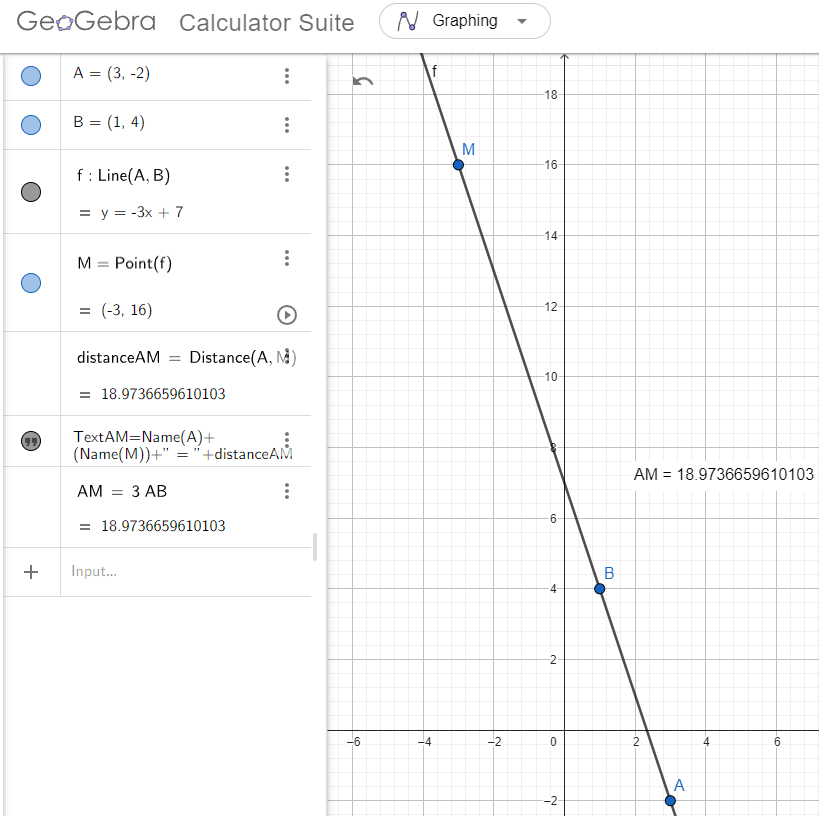
\includegraphics[height=4.4cm,width=1\textwidth,keepaspectratio]{resources/geogebra.png}
                    \caption*{\href{https://www.geogebra.org/calculator}{Link to the Geogebra}}
                    \label{fig:resources/geogebra.png}
                \end{figure}
            \end{column}
        \end{columns}
    }
\end{frame}

\begin{frame}[t]{Task 5 and 6}
    \framesubtitle{}
    \textbf{5.} Find the coordinates of the gravity center of a triangular plate $\mathbf{ABC}$ with vertices in points $\mathbf{A}(3,1), \mathbf{B}(6,3), \mathbf{C}(0,2)$. \bigskip

    \textbf{6.} In the plane of the triangle $ \mathbf{ABC}$ find the point $ \mathbf{O}$ such that $\overrightarrow{OA} + \overrightarrow{OB} + \overrightarrow{OC} = \mathbf{0}$. Are there such points outside of the triangle? \\
    \textit{Note}: $ \mathbf{0}$ is a zero-vector. \\
\end{frame}

\begin{frame}[t]{Center of gravity VS Center of mass}
    \framesubtitle{}
    For classical mechanics - it’s the same. More info \href{https://www.youtube.com/watch?v=abUFbZfPzjY}{here}
\end{frame}

\begin{frame}[t]{Where a center of mass can be used?}
    \framesubtitle{}
    \begin{figure}[H]
        \begin{subfigure}{0.49\textwidth}
            \centering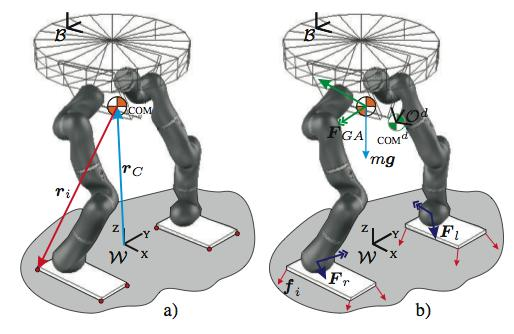
\includegraphics[height=6cm,width=1\textwidth,keepaspectratio]{resources/image35.png}
            % \caption{capture1}
            \label{fig:resources/image35.png}
        \end{subfigure}
        \begin{subfigure}{0.49\textwidth}
            \centering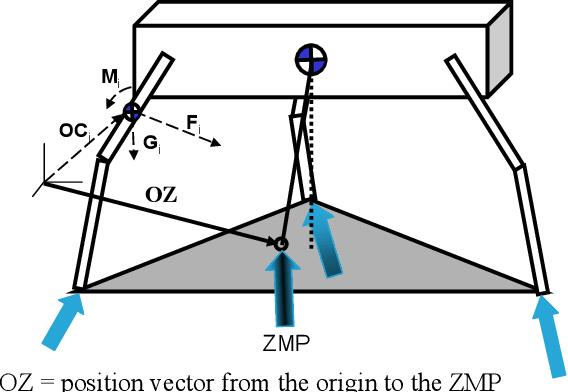
\includegraphics[height=6cm,width=1\textwidth,keepaspectratio]{resources/image36.png}
            % \caption{capture2}
            \label{fig:resources/image36.png}
        \end{subfigure}
    \end{figure}
\end{frame}

\begin{frame}[t]{How to find a CoM in real life}
    \framesubtitle{}
    \vspace{-0.3cm}
    \begin{figure}[H]
        \centering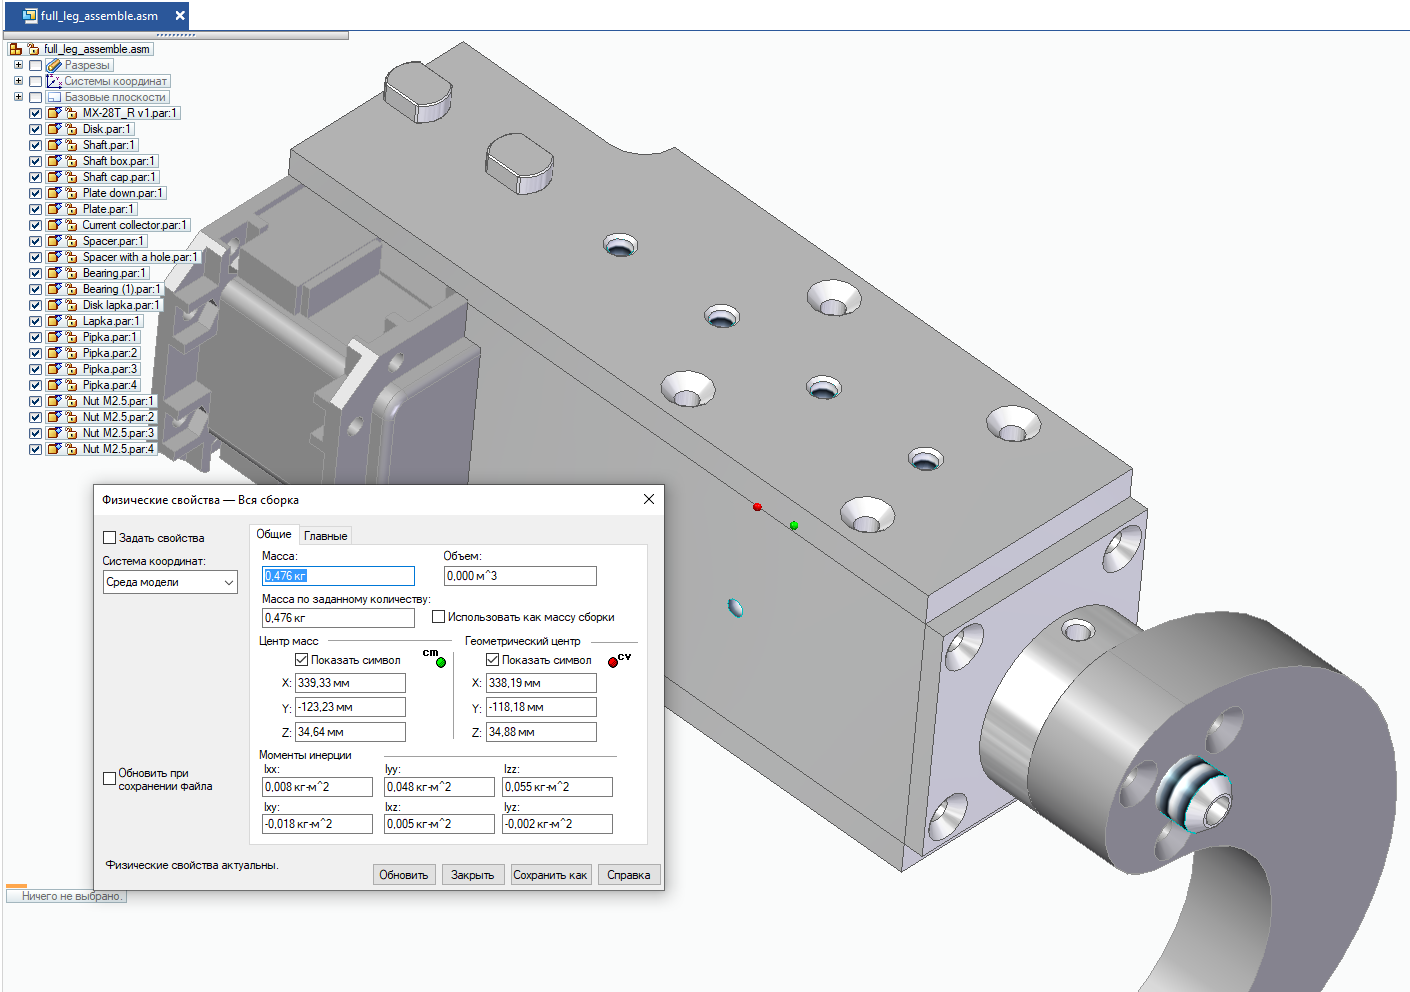
\includegraphics[height=6cm,width=1\textwidth,keepaspectratio]{resources/image37.png}
        \label{fig:resources/image37.png}
    \end{figure}
\end{frame}

\begin{frame}[t]{Task 5}
    \framesubtitle{Solution made in CAD}
    \vspace{-0.6cm}
    \begin{figure}[H]
        \centering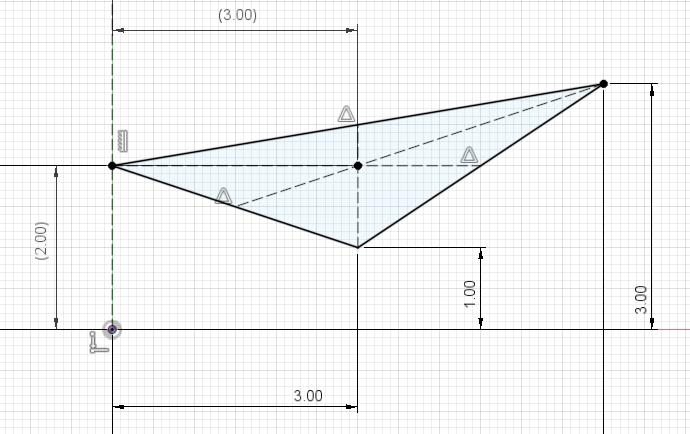
\includegraphics[height=6cm,width=1\textwidth,keepaspectratio]{resources/image39.png}
        \label{fig:resources/image39.png}
    \end{figure}
\end{frame}

\begin{frame}[t]{Subspace}
    \framesubtitle{}
    \begin{exampleblock}{Definition}
        $W$ is a \underline{subspace} of $V$ if

        \begin{tabular}{lll}
            a) & $W \subset V$                                                                 & (subset)                 \\
            b) & $\mathbf{u},\mathbf{v}\in W \Rightarrow \mathbf{u}+\mathbf{v} \in W$          & (closure under addition) \\
            c) & $\mathbf{u}\in W, \lambda \in \mathbb{R} \Rightarrow \lambda \mathbf{u}\in W$ &
            (closure under scalar multiplication)
        \end{tabular}
    \end{exampleblock}
\end{frame}

\begin{frame}[t]{Task 7}
    \framesubtitle{}
    Check for each case if the following set of vectors is a subspace or not. Explain your answer. \\
    1. Part of the plane $x > 0$ \\
    2. Entire plane \\
    3. Part of the plane $y < 0$ \\
    4. Part of the plane $x > 0, \; y > 0$  \\
    5. Inner circle with the radius $r = 5$ \\
\end{frame}

\begin{frame}[t]{Reference material}
    \framesubtitle{OnlineMschool}
    \begin{itemize}
        \item \href{https://youtu.be/fNk_zzaMoSs}{Vectors | Chapter 1, Essence of linear algebra - YouTube}
        \item \href{https://youtu.be/k7RM-ot2NWY}{Linear combinations, span, and basis vectors | Chapter 2, Essence of linear algebra - YouTube}
        \item \href{https://onlinemschool.com/math/library/vector/vector-definition/}{Vectors Definition. Main information}
        \item \href{http://www.mathprofi.ru/vektory_dlya_chainikov.html}{Векторы для чайников. Действия с векторами. Координаты вектора.}
        \item \href{http://www.mathprofi.ru/linejnaja_nezavisimost_vektorov_bazis_vektorov.html}{Линейная зависимость и независимость векторов. Базис векторов}
    \end{itemize}
\end{frame}

\fbckg{fibeamer/figs/last_page.png}
\frame[plain]{}

\end{document}